\documentclass[tikz,border=2mm]{standalone}

\begin{document}
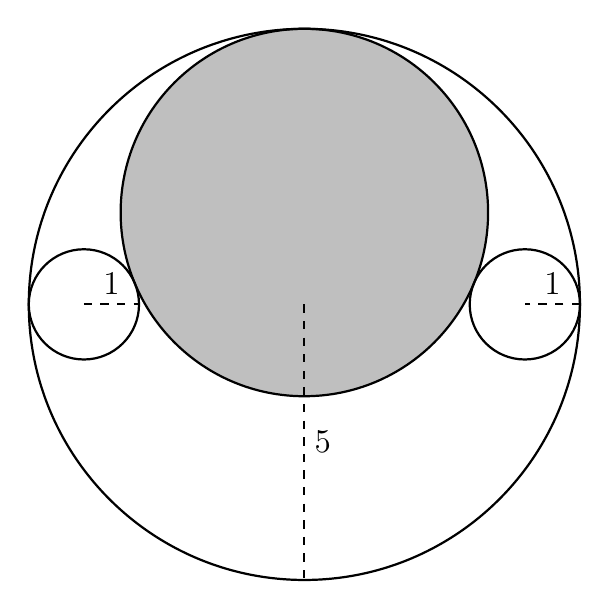
\begin{tikzpicture}[scale=0.7,every node/.style={font=\large},thick]
  \pgfmathsetmacro\x{5}
  \pgfmathsetmacro\y{3.33333}
  \pgfmathsetmacro\z{1}
  % larger of the inscribed circles:
  \draw[fill=gray!50] (0,\x-\y) circle (\y);
  % small inscribed circles:
  \draw (-\x+\z,0) circle (\z);
  \draw (\x-\z,0) circle (\z);
  % radius of small circles:
  \draw[dashed] (-\x+\z,0) --++ (\z,0) node[midway,above] {$1$};
  \draw[dashed] (\x,0) --++ (-\z,0) node[midway,above] {$1$};
  % large circle:
  \draw (0,0) circle (\x);
  % radius of large circle:
  \draw[dashed] (0,0) --++ (0,-\x) node[midway,right] {$5$};
\end{tikzpicture}
\end{document}


